\chapter{Experiments} \label{chapt:Experiments}

In this section, we describe three groups of experiments conducted to evaluate ASSIM. The first group examines the computational costs of ASSIM, time and memory use. The second group evaluates the accuracy of BSC and RCDA by recording their precision and recall values under difference circumstances. Lastly, we inject different kinds of drifts into the data streams and test the efficiency and accuracy of our drift detector. 

All experiments are conducted on a machine with Intel Core i7-7700 Desktop Processor 4 Cores with up to 4.2 GHz CPU with 32GB RAM.


\section{Descriptions of the Datasets}

\begin{table}[h!]
\caption{Descriptions of the Datasets}
\label{tb:datasets}
\begin{center}
\addtolength{\tabcolsep}{4.0pt}
\begin{tabular}{ll}
    \toprule
    \multirow{1}{*}{Dataset} &
      \multicolumn{1}{l}{Description} \\
      \midrule
    T10I1KD100K & {synthetic dataset with an average transaction length 10}  \\
    T15I1KD1M & {synthetic dataset with an average transaction length 15}  \\
    mushrooms & {prepared based on the UCI mushrooms dataset}  \\
    retail & {retail market basket data from a Belgian retail store}\\
    pumsb & {census data for population and housing}\\
    chess & {prepared based on the UCI chess dataset}\\
    connect & {prepared based on the UCI connect-4 dataset}\\
    accidents & {anonymized traffic accident data}\\
    BMS\_WebView & {click-stream data from a webstore used in KDD-Cup 2000}\\
    chainstore &  {customer transactions from a retail store from NU-Mine Bench}\\
    \bottomrule
\end{tabular}
\end{center}
\end{table}
We employed ten datasets including eight of the largest attribute-value datasets from the UCI machine learning \cite{uci1,uci2} and UCI KDD \cite{uci3} repositories together with the BMS-WebView \cite{bms}, retail \cite{retail} and chainstore from CUCIS\cite{CUCIS} datasets. The other two are synthetic datasets created by IBM data generator. These datasets are described in Table \ref{tb:datasets}. % and Table \ref{tb:datades}.

Each synthetic dataset configuration (\textit{T10I1KD100K} and \textit{T15I1KD1M}) was generated with different seed values and passed into the algorithm 30 times. The other eight real-world datasets were tested a single time each.
% \begin{table}[h!]
% \caption{Dataset Description}
% \label{tb:datades}
% \begin{center}
% \begin{tabular}{lrr}
%     \toprule
%     \multirow{1}{*}{Dataset} &
%       \multicolumn{1}{r}{Record} &
%       \multicolumn{1}{r}{Item} \\
%       \midrule
%     T10I1KD100K & {100,000} & {1,000} \\
%     T15I1KD1M & {1,000,000}& {1,000}\\
%     mushrooms & {8,416} & {119}\\
%     retail & {88,162} & {16,470}\\
%     pumsb & {49,046} & {2,113}\\
%     chess & {3,196} & {75}\\
%     connect & {67,557} & {129}\\
%     accidents & {340,183} & {468}\\
%     BMS\_WebView\_1 & {59,602} & {497}\\
%     chainstore & {1,112,949} & {46,086}\\
%     \bottomrule
% \end{tabular}
% \end{center}
% \end{table}

\section {Runtime and Memory Performance}
We ran our ten datasets on BSC and SSIG separately to record the time and memory used for each component of our technique. In this case, SSIG without batches represents the ground truth which produces the truth result of Self-Sufficient itemsets in each dataset.

Table \ref{tb:time1} %and Table \ref{tb:time2} 
illustrate that BSC works as a stable technique. It has a faster runtime performance as compared from SSIG without batches. In our experiments, the tolerance error rate for the approximation $e=0.05$ and frequency difference threshold $\tau=25\%$.
To further evaluate the efficiency of BSC, we also perform two additional experiments for each dataset. In the additional set of experiments, we feed equally divided batches into SSIG (divided into the same amount of batches as BSC but in fixed interval). This is to show how runtime and memory performance is effected given the same number of datasets. In the second set of experiments, we feed batches into SSIG separately based on the pre-detemined size of the  intervals found using BSC. To do this we noted the location of the batch size found in BSC and then superimposed the same exact batch sizes for SSIG. The significance level $\alpha=0.05$ was used for performing Fisher's Exact Test in SSIG.

This experiments was to evaluate the runtime and memory if we mined at the same time point of BSC.
Table \ref{tb:time1}  shows us that there is no significant difference between the time and memory consumption between SSIG with a fixed interval and with pre-calculated batches based  found using BSC. 

\begin{table}[h!]
\caption{Runtime and Memory Performance}
\label{tb:time1}
\begin{center}
\addtolength{\tabcolsep}{5.0pt}
\begin{tabular}{lrrrr}
    \toprule
    \multirow{2}{*}{Dataset} &
      \multicolumn{2}{c}{BSC} &
      \multicolumn{2}{c}{SSIG without batches} \\
      & {Time (s)} & {Memory (Mb)} & {Time (s)} & {Memory (Mb)} \\
      \midrule
    T10I1KD100K & \textbf{\(1.97\pm 0.92\)} & {\(210.28\pm 0.89\)} & {\(2.85\pm 0.33\)} & {\(148.41\pm 0.33\)} \\
    T15I1KD1M & \textbf{\(35.24\pm 1.36\)} & {\(642.81\pm 2.01\)} & {\(47.42\pm 3.64\)} & {\(572.22\pm 0.97\)} \\
    mushrooms & \textbf{\(0.54\pm 0.04\)} & {\(78.36\pm 0.27\)} & {\(1.09\pm 0.16\)} & {\(55.73\pm 0.21\)} \\
    retail & \textbf{\(1.64 \pm 0.29\)} & {\(192.45\pm 0.84\)}& {\(2.44\pm 1.02\)} & {\(136.85\pm 0.76\)}\\
    pumsb & \textbf{\(0.92\pm 0.05\)} & {\(101.34\pm0.76\)}& {\(1.49\pm0.11\)} & {\(74.32\pm 0.19\)}\\
    chess & \textbf{\(0.19\pm0.02\)} & {\(25.92\pm0.37\)}& {\(0.31\pm0.10\)} & {\(10.78\pm0.14\)}\\
    connect & \textbf{\(1.85\pm 0.06\)} & {\(168.32\pm1.92\)}& {\(2.11\pm 0.21\)} & {\(103.27\pm0.35\)}\\
    accidents & \textbf{\(8.24\pm0.79\)} & {\(385.56\pm2.34\)}& {\(2.87\pm0.67\)} & {\(339.14\pm0.68\)}\\
    BMS\_WebView & \textbf{\(1.11\pm0.12\)} & {\(119.38\pm0.78\)}& {\(1.46\pm0.40\)} & {\(91.25\pm0.07\)}\\
    chainstore & \textbf{\(38.21\pm1.28\)} & {\(783.15\pm2.35\)}& {\(51.97\pm2.07\)} & {\(711.92\pm1.06\)}\\
    \bottomrule
\end{tabular}
% \end{center}
% \end{table}

\noalign{\smallskip}

% \begin{table}[h!]
% \caption{Time and Memory Use}
% \label{tb:time2}
% \begin{center}
\begin{tabular}{lrrrr}
    \toprule
    \multirow{2}{*}{Dataset} &
      \multicolumn{2}{c}{SSIG with fixed intervals} &
      \multicolumn{2}{c}{SSIG with batches} \\
      & {Time (s)} & {Memory (Mb)} & {Time (s)} & {Memory (Mb)} \\
      \midrule
    T10I1KD100K & {\(3.04\pm 0.69\)} & {\(149.12\pm 0.30\)} & {\(3.05\pm 0.23\)} & {\(149.10\pm 0.27\)} \\
    T15I1KD1M & {\(49.10\pm 2.41\)} & {\(574.11\pm 0.85\)} & {\(49.17\pm 1.94\)} & {\(574.12\pm 0.88\)} \\
    mushrooms & {\(1.15\pm 0.11\)} & {\(56.09\pm 0.33\)} & {\(1.17\pm 0.23\)} & {\(56.12\pm 0.19\)} \\
    retail & {\(2.69 \pm 0.27\)} & {\(138.02\pm 0.81\)}& {\(2.82\pm 0.04\)} & {\(137.98\pm 0.84\)}\\
    pumsb & {\(1.52\pm 0.11\)} & {\(75.65\pm0.22\)}& {\(1.52\pm0.12\)} & {\(75.61\pm 0.27\)}\\
    chess & {\(0.39\pm0.02\)} & {\(10.98\pm0.07\)}& {\(0.39\pm0.04\)} & {\(11.02\pm0.08\)}\\
    connect & {\(2.30\pm 0.10\)} & {\(104.25\pm0.29\)}& {\(2.28\pm0.09\)} & {\(104.23\pm0.33\)}\\
    accidents & {\(3.02\pm0.32\)} & {\(321.01\pm0.72\)}& {\(2.99\pm0.17\)} & {\(320.88\pm0.77\)}\\
    BMS\_WebView & {\(1.57\pm0.07\)} & {\(92.07\pm0.15\)}& {\(1.57\pm0.12\)} & {\(92.05\pm0.17\)}\\
    chainstore & {\(56.39\pm0.27\)} & {\(714.24\pm0.84\)}& {\(56.41\pm0.19\)} & {\(714.25\pm0.86\)}\\
    \bottomrule
\end{tabular}
\end{center}
\end{table}




\section{Experiments to Evaluate Precision and Recall}
As a result of using Lossy Counting \cite{lossy} in BSC, all the frequent items produced by BSC are true positives. Thus producing 100\% precision. Lossy Counting in BSC only provides an approximation to the frequency of an items a batch. Some of the frequent items, which should have been included for expansion to Self-Sufficient itemsets may be missed. This would lead to  recall being less than 100\%. We use the SSIG without batches as the ground truth of the set of self-sufficient itemsets found. 

\begin{table}[h!]
\caption{Precision and Recall}
\label{tb:pr1}
\begin{center}
\resizebox{\textwidth}{!}{
\begin{tabular}{lrrrrrr}
    \toprule
    \multirow{2}{*}{Dataset} &
    \multicolumn{2}{c}{BSC} &
      \multicolumn{2}{c}{SSIG with fixed intervals} &
      \multicolumn{2}{c}{SSIG with batches} \\
  & {Precision (\%)} & {Recall (\%)}
      & {Precision (\%)} & {Recall (\%)}& {Precision (\%)} & {Recall (\%)} \\
      \midrule
    T10I1KD100K & {\(100\%\pm 0\%\)} & {\(97\%\pm 2\%\)}& {\(96\%\pm 1\%\)} & {\(98\%\pm 2\%\)}& {\(97\%\pm 2\%\)} & {\(98\%\pm 1\%\)} \\
    T15I1KD1M & {\(100\%\pm 0\%\)} & {\(98\%\pm 1\%\)} &{\(93\%\pm 3\%\)} & {\(95\%\pm 4\%\)} & {\(96\%\pm 2\%\)} & {\(99\%\pm 1\%\)} \\
    
    \noalign{\smallskip}\hline\noalign{\smallskip}
    
    mushrooms & {\(100\%\)} & {\(97\%\)} &{\(97\%\)} & {\(99\%\)} & {\(97\%\)} & {\(97\%\)}\\
    retail & {\(100\%\)} & {\(98\%\)} &{\(95\%\)} & {\(96\%\)} & {\(97\%\)} & {\(97\%\)}\\
    pumsb & {\(100\%\)} & {\(98\%\)} &{\(96\%\)} & {\(94\%\)} & {\(97\%\)} & {\(94\%\)}\\
    chess & {\(100\%\)} & {\(100\%\)} &{\(100\%\)} & {\(98\%\)} & {\(100\%\)} & {\(99\%\)}\\
    connect & {\(100\%\)} & {\(98\%\)} & {\(95\%\)} & {\(97\%\)} & {\(95\%\)} & {\(97\%\)}\\
    accidents &{\(100\%\)} & {\(96\%\)} &  {\(93\%\)} & {\(94\%\)} & {\(98\%\)} & {\(98\%\)}\\
    BMS\_WebView & {\(100\%\)} & {\(99\%\)} &{\(96\%\)} & {\(95\%\)} & {\(99\%\)} & {\(97\%\)}\\
    chainstore & {\(100\%\)} & {\(95\%\)} &{\(95\%\)} & {\(97\%\)} & {\(96\%\)} & {\(99\%\)}\\
    \bottomrule
\end{tabular}}
\end{center}
\end{table}


With the batch calculation from BSC, the correctly detected batches of data stream achieved better precision and recall values for Self-Sufficient itemset mining as compared to SSIG with fixed intervals or SSIG with batches.

\section {Experiments to Evaluate the Regional Drift Detection}
In the drift detection part, we perform two different tests: abrupt and gradual drift detection on \textit{T10I1KD100K} dataset. The delta value $\delta=0.002$ was set for ADWIN drift detector. For abrupt drifts, we inject different numbers of abrupt drifts, specifically 5, 10 and 20 into \textit{T10I1KD100K}. Several indications were recorded: time and memory costs, true and false positives, and delay. Based on the results the increase of  drift points, this leads to worse false positives.

To evaluate gradual drift detection, we used the same dataset \textit{T10I1KD100K} but changed data in different rates noted as the slopes, specifically 250, 500 and 1,000. Same indications were used for this test, and it showed that higher slopes produce worse false positives and longer delay.

\begin{table}[h!]
\caption{Abrupt Drift Detection}
\label{tb:abrupt}
\begin{center}
\resizebox{\textwidth}{!}{
\begin{tabular}{lrrrrr}
    \toprule
    \multirow{1}{*}{\#Drifts} &
      \multicolumn{1}{c}{Time (s)} &
      \multicolumn{1}{c}{Memory (Mb)} &
      \multicolumn{1}{c}{TP Rate (\%)} &
      \multicolumn{1}{c}{FP} &
      \multicolumn{1}{c}{Delay}\\
      \midrule
    5 & {\(6.42\pm 0.11\)} & {\(23.1\pm 0.07\)} & {\(1.0\pm 0.00\)} & {\(77.81\pm 0.07\)} & {\(184.65\pm 67.84\)}\\
    10 & {\(6.54\pm 0.08\)} & {\(23.2\pm 0.09\)} & {\(1.0\pm 0.00\)} & {\(385.42\pm 39.61\)} & {\(157.82\pm 39.61\)}\\
    20 & {\(6.59\pm 0.10\)} & {\(23.1\pm 0.08\)} & {\(1.0\pm 0.00\)} & {\(793.11\pm 55.28\)} & {\(93.11\pm 35.28\)}\\
    \bottomrule
 \end{tabular}
 }
\end{center}
\end{table}


\begin{table}[h!]
\caption{Gradual Drift Detection}
\label{tb:gradual}
\begin{center}
\resizebox{\textwidth}{!}{
\begin{tabular}{lrrrrr}
    \toprule
    \multirow{1}{*}{Slope} &
      \multicolumn{1}{c}{Time (s)} &
      \multicolumn{1}{c}{Memory (Mb)} &
      \multicolumn{1}{c}{TP Rate (\%)} &
      \multicolumn{1}{c}{FP} &
      \multicolumn{1}{c}{Delay}\\
      \midrule
    250 & {\(6.52\pm 0.14\)} & {\(23.1\pm 0.03\)} & {\(1.0\pm 0.00\)} & {\(174.29\pm 53.11\)} & {\(98.35\pm 78.25\)}\\
    500 & {\(6.82\pm 0.18\)} & {\(23.2\pm 0.07\)} & {\(1.0\pm 0.00\)} & {\(482.36\pm 42.83\)} & {\(164.70\pm 69.83\)}\\
    1000 & {\(7.01\pm 0.22\)} & {\(23.1\pm 0.03\)} & {\(1.0\pm 0.00\)} & {\(853.16\pm 107.28\)} & {\(218.65\pm 109.62\)}\\
    \bottomrule
 \end{tabular}
 }
\end{center}
\end{table}

\section{Case Study: USCensus}

This dataset is transformed from the US Census 1990 dataset, obtained from UCI Machine Learning Repository~\cite{uci1,uci2}, where 1,000,000 instances were transformed to transactions, and where there are 396 distinct items. Figure \ref{fig:frequs} shows the normalised item frequency distribution of the USCensus dataset. When we compared the distribution of the USCensus dataset, to other commonly used data mining datasets, we observed that the USCensus dataset is much more sparse in nature compared to the other real-world datasets we used to perform experiments, but more dense than datasets like Kosarak. Because of its sparsity, it is interesting to see how this could potentially affect the Self-Sufficient itemset mining process. 

\begin{figure}[H]
    \centering
    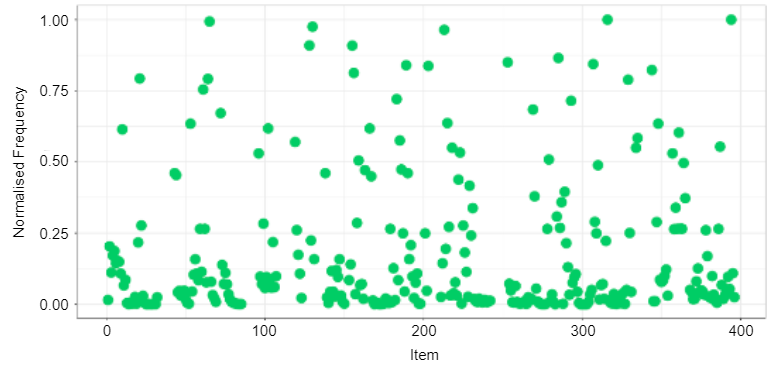
\includegraphics[width=0.9\textwidth]{Experiments/Frequencynor.png}
    \caption{Normalised item frequency distribution}
    \label{fig:frequs}
\end{figure}

\subsection{Runtime and Memory Performance}
We ran USCensus on BSC and SSIG separately to record the time and memory used for each component of our technique. Table \ref{tb:time2} illustrates that for a very sparse dataset like USCensus, BSC with SSIG may need a longer time to divide batches but the difference before and after adding BSC is not very significant.

\begin{table}[h!]
\caption{Runtime and Memory Performance for USCensus}
\label{tb:time2}
\begin{center}
\addtolength{\tabcolsep}{5.0pt}
\begin{tabular}{lrrrr}
    \toprule
    \multirow{2}{*}{Dataset} &
      \multicolumn{2}{c}{BSC} &
      \multicolumn{2}{c}{SSIG without batches} \\
      & {Time (s)} & {Memory (Mb)} & {Time (s)} & {Memory (Mb)} \\
      \midrule
    USCensus & \textbf{\(32.81\pm 0.94\)} & {\(654.27\pm 3.11\)} & {\(32.25\pm 1.63\)} & {\(584.74\pm 1.16\)} \\
    \bottomrule
\end{tabular}


\noalign{\smallskip}

\begin{tabular}{lrrrr}
    \toprule
    \multirow{2}{*}{Dataset} &
      \multicolumn{2}{c}{SSIG with fixed intervals} &
      \multicolumn{2}{c}{SSIG with batches} \\
      & {Time (s)} & {Memory (Mb)} & {Time (s)} & {Memory (Mb)} \\
      \midrule
    USCensus & {\(33.71\pm 1.22\)} & {\(661.32\pm 0.51\)} & {\(33.25\pm 0.43\)} & {\(659.10\pm 0.44\)} \\
    \bottomrule
\end{tabular}
\end{center}
\end{table}

\subsection{Experiments to Evaluate Precision and Recall}

Same as we discussed before, the results came out from BSC are guaranteed to be frequent which guarantees a 100\% precision. Because most of the items in USCensus are infrequent with a less than 0.1 frequency, the recall of BSC performs well - very frequent items are easy to be found. 

BSC provides specific calculations on the distribution change points for frequent items which directly help SSIG with the Self-Sufficient itemset mining process. According to \ref{tb:prrc}, these properly divided batches of USCensus achieved a much better precision and recall values for Self-Sufficient itemset mining comparing to the ground truth (SSIG with fixed intervals).

\begin{table}[h!]
\caption{Precision and Recall for USCensus}
\label{tb:prrc}
\begin{center}
\resizebox{\textwidth}{!}{
\begin{tabular}{lrrrrrr}
    \toprule
    \multirow{2}{*}{Dataset} &
    \multicolumn{2}{c}{BSC} &
      \multicolumn{2}{c}{SSIG with fixed intervals} &
      \multicolumn{2}{c}{SSIG with batches} \\
  & {Precision (\%)} & {Recall (\%)}
      & {Precision (\%)} & {Recall (\%)}& {Precision (\%)} & {Recall (\%)} \\
      \midrule
    USCensus & {\(100\%\)} & {\(97\%\)} &{\(92\%\)} & {\(95\%\)} & {\(96\%\)} & {\(98\%\)}\\
    \bottomrule
\end{tabular}}
\end{center}
\end{table}


\section{Conclusion}

In this section I conducted several experiments to test the performance of ASSIM by comparing the runtime and memory use, precision and recall rates and drift detection accuracy. From the runtime and memory experiments, I concluded that there is no significant difference between the time and memory consumption between with or without using Batch Size Calculator, which shows ASSIM does not requires extra computation cost. I then evaluated the precision and recall rates, data stream with correctly divided batches achieved better precision and recall values for Self-Sufficient itemset mining than using no ASSIM. Finally, I tested our regional drift detector which also achieved promising results. My case study on US Census data also showed similar results as before, proved that ASSIM works as a stable and workable framework.

